\documentclass[
    english, % Klasei padavus parametrą 'english', darbas bus anglų kalba.
    % signatureplaces % prideda parašų vietas tituliniame puslapyje
]{VUMIFPSkursinis}
\usepackage{float}
\usepackage{wrapfig2}
\usepackage{hyperref}
\usepackage{algorithmicx}
\usepackage{algorithm}
\usepackage{algpseudocode}
\usepackage{amsfonts}
\usepackage{amsmath}
\usepackage{bm}
\usepackage{caption}
\usepackage{color}
\usepackage{graphicx}
\usepackage{listings}
\usepackage{subcaption}
\usepackage{biblatex}
\usepackage{geometry}
\usepackage{booktabs}
\usepackage{multirow}
\usepackage{diagbox}
\usepackage{afterpage}
\usepackage{makecell}
\usepackage[inkscapelatex=false]{svg}
\renewcommand{\cftdotsep}{1} 


% Titulinio aprašas
\university{Vilnius university}
\faculty{Faculty of mathematics and informatics}
\department{Software engineering study program}
\papertype{Software Engineering II laboratory work 2}
\title{EduPal change request analysis, requirements and project plan}
\status{2 course 5 group students}
\author{Motiejus Šveikauskas}
\secondauthor{Kanstantinas Piatrashka}
\thirdauthor{Aldas Vertelis}
\fourthauthor{Danielius Podbielski}
\reviewer{doc. dr. Vardauskas Pavardauskas}
\date{Vilnius – \the\year}

\bibliography{bibliografija}

\begin{document}
\maketitle

\tableofcontents

\section{Context}

EduPal is a learning aid business which helps both students and teachers by allowing educators to conveniently upload course information for students to learn. EduPal offers unique features such as pomodoro timer, note creation and export in pdf, setting goals, chatGPT integration. EduPal lets users have subjects, create topics inside subjects and upload conspectuses.

\subsection{Change request}

\textbf{User need:} Students want to revise learned material in interactive and efficient way. We propose an idea to integrate quizzes into the system. Every topic should have a quiz section where topic owner  should be able to create, update and delete quizzes. Quiz consists of randomly shuffled questions, question answer interface should be simple and easy to use with mouse or touch device. Upon answering a question, student gets an instant feedback.

\vspace{\baselineskip}

Currently EduPal system offers no way to revise or test knowledge of a particualr topic. It is responsibility of users to check their own understanding of material by using their own aproach which takes more time than they would like and adds a complexity of choosing a third party service or methodology. Integrating quizzes into a system would boost engagement of users and simplify their studying process.

\subsection{Change priority}

Majority of students need to use EduPal with third party active learning tool that provides feedback (typically flashcard or quiz platform). Many major players (such as Quizlet and Kahoot) do not yet have proper conspectus storage system such as EduPal, meaning that users of those platforms tend to rely on solutions such as EduPal. Implementing quizzes can motivate active learning tool users to try EduPal while some may decide that only EduPal is enough for their needs. Additionaly, active learning tool platforms may implement data storage and sharing system similar to EduPal that would result in users migrating away from EduPal. Benefits of built in quiz capability include:

\begin{enumerate}
    \item EduPal can be treated as all-in-one system
    \item Users will not need to search for and configure third party systems
    \item EduPal can be advertised to a broader user base.
    \item Quizzes would also provide valuable data insights into user engagement and performance, which could be used for strategic decisions by managers.
\end{enumerate}

And drawbacks are:

\begin{enumerate}
    \item Being all-in-one system, EduPal will have to compete with both conspectus storage systems and active learning tool systems which requires more financial investements
    \item Some users will not want to use EduPal solution as they are acustomed to their setups
\end{enumerate}

We consider this change priority to be \textbf{medium to high}.

\subsection{Affected stakeholders}

The feature would affect these stakeholders:

\begin{enumerate}
    \item Teachers would get the opportunity to emphasize more important questions by creating quizzes and would have the chance to provide more helpful material in a different format.
    \item Students would have the opportunity to learn in an easier and more useful way. The opportunity to test their own knowledge would allow students to realize which topics they know well and on which topics they should revise.
    \item Developers and Maintainers would have to create, test and maintain the feature.
    \item Marketers would have to advertise the feature.
    \item Business owners and Investors will likely see increase in user base and profits.
\end{enumerate}

\subsection{Implementation alternatives}

\subsubsection{First option: use notes to provide links to third party quiz service}

This simple implementation alternative requires no implementation whatsoever.  We would create a note with a link to another website, where a new user account would have to be created if the student is using the app for the first time, otherwise logging in is sufficient. Once authenticated the student will be presented with the quiz they wished to take.

\textbf{Duration:} 1 day. Most of the time being consumed by searching for a suitable third-party app.

\textbf{Pricing:} This option will not cost our client anything if they find the suitable third-party app themselves, otherwise, if we are tasked with determining the most suitable third-party app, this implementation will cost a trivial sum.

\textbf{User impact:} High. The disadvantage of this approach is that both the teachers and the students will be forced to create a new account in a separate application.

\textbf{Scalability:} Not scalable. Meaning we can not add new features or change existing ones

\textbf{Maintenance:} We do not have to maintain it as it falls upon the owners of the third-party quiz app, saving us money and time as a result.

\subsubsection{Second option: integrate third-party API}

This option is a middle ground between the first and the third option detailed below. Our team proposes integrating a third-party quizzing app into our system through an API, perhaps even establishing a potential partnership with a suitable quizzing app. This implementation would feature a button on every topic which would take users to a new tab or a window and immediately begin the quiz with no authorization required. If needed, quiz scores could be stored in our system and displayed to the user.

\textbf{Duration:} 2-4 weeks, including time for developing quiz buttons, understanding the API, and establishing potential partnerships.

\textbf{Pricing:} 5-10k euros. This option incurs higher costs due to the need for developers, testers, a designer, and software engineers working on the feature for 2-3 weeks.

\textbf{User impact:} Medium. Users benefit from not having to create separate accounts or navigate to another webpage, though they may encounter mismatched UI elements and occasional performance issues.

\textbf{Scalability:} Limited scalability, as we lack control over the third-party API, restricting our ability to make extensive changes.

\textbf{Maintenance:} Increased maintenance demands due to shared functionality ownership and the need to keep up with API changes.

\subsubsection{Third option: add quiz subsystem to EduPal}

In our chosen implementation, our team implements a fully fledged quizzing feature in the EduPal system. In this option our team would develop the quiz app embedded in EduPal with its own API and frontend choices.

\textbf{Duration:} 1-2 months for full implementation, including development and testing.

\textbf{Pricing:} >10k euros. This option is the most costly due to the need for a dedicated team of developers and testers.

\textbf{User impact:} Low. Users can seamlessly access the quiz feature within EduPal without complications.

\textbf{Scalability:} Highly scalable as our team maintains complete control over the system, allowing for future enhancements and quick resolution of any issues.

\textbf{Maintenance:} The addition of a new service increases maintenance challenges, but it enables greater flexibility and autonomy in addressing any concerns.

\subsection{Implementations comparison}

\begin{figure}[ht]
    \centering
    \begin{tabular}{|c|c|c|c|}
        \hline
                                & First option & Second option & Third option \\
        \hline
        Duration                & 1 day        & 2-4 weeks     & 1-2 months   \\
        \hline
        Cost                    & 0            & 5-10k euros   & >10k euros   \\
        \hline
        User impact             & High         & Medium        & Low          \\
        \hline
        Scalability/Maintenance & Low/Low      & Low/Medium    & High/High    \\
        \hline
    \end{tabular}
    \caption{Implementations comparison}
    \label{tab:implementations-comparison}
\end{figure}

\subsection{Outsourcing capability}

Although outsourcing the feature to other developers might help save time and be an easier option, we decided to build the feature in house. We would have complete control of how our feature would look and work. Also, this way we would avoid any dependencies on third-party services, maintain current application efficiency, and save capital.

\subsection{Project management}

We put our business team as core management of the project. They must ensure that the product acknowledges end user needs, control the budget and execution time, handle advertisement of the feature. Development team must follow business team decision, however developers need to ensure that quiz integration will not have performance or maintenance imapct on other parts of the system and will not result in technical debt.

\section{Domain model}

\begin{figure}[ht]
    \centering
    \includegraphics[width=\textwidth]{../lab3diags/domain.drawio.png}
    \caption{Domain model diagram}
    \label{domain-model}
\end{figure}

\begin{description}
    \item[User] Every EduPal customer is user - they are able to create subjects, topics, upload conspectuses, rate them and so on.
    \item[Topic owner] User who owns a particular topic - only they are able to edit its contents, including quizzes.
    \item[Topic] A part of subject (not related to change request). Topic consists of conspectuses, comments and quizzes.
    \item[Quiz] A named collection of questions
    \item[Question] Question has a name and a set of incorrect options as well as correct one.
    \item[Option] Question option is a text answer.
    \item[Quiz session] Users start quiz session when they take the quiz.
    \item[Quiz session question] Questions are shufled during quiz session.
    \item[Question feedback] Feedback whether question answer is correct or not.
    \item[User answer] User answer is an option that was picked by user.
\end{description}

\section{Use cases}

\subsection{List quizzes}

\begin{figure}[ht]
    \centering
    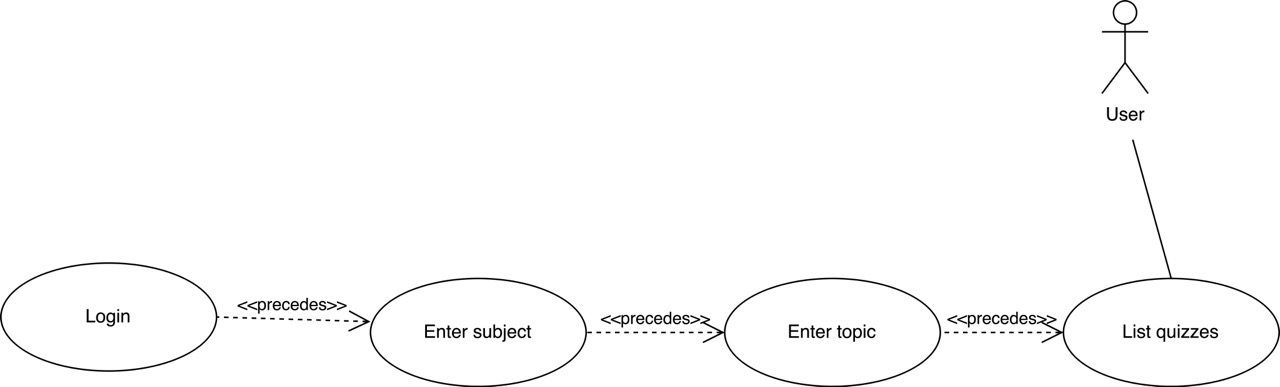
\includegraphics[width=\textwidth]{../lab3diags/list.drawio Large.jpeg}
    \caption{List quizzes use case}
    \label{list-quizzes}
\end{figure}

\noindent\textbf{\fontsize{13}{15}\selectfont Main scenario:}

\textit{The user} opens the EduPal website; the system displays the Login Page. \textit{The user} enters login information and clicks the Login Button; the system verifies identity of \textit{the user}, initiates the user session, and shows the Subject List Page. \textit{The user} clicks on a specific subject; the system loads its \textit{topics} and shows the Topic List Page for that subject. \textit{The user} clicks on a specific topic; the system loads \textit{topic} data and shows the Topic Page. \textit{The user} clicks the Quizzes Button; the system fetches a list of \textit{quizzes} associated with \textit{the topic} and shows a Quiz List page. \textit{The user} clicks on the particular \textit{quiz}; the system displays the Quiz Page.

\noindent\textbf{\fontsize{13}{15}\selectfont Alternatives:}

\textbf{\textit{The user} enters incorrect login information:} The system displays the Login Failed Message.

\textbf{\textit{User} session expired:} The system navigates \textit{the user} to the Login Page.

\textbf{\textit{The user} is \textit{the topic owner}} The system shows the Create Quiz button on the Quiz List Page. The system shows Edit and Delete Buttons on the Quiz Page.

\pagebreak

\subsection{Take the quiz}

\begin{figure}[ht]
    \centering
    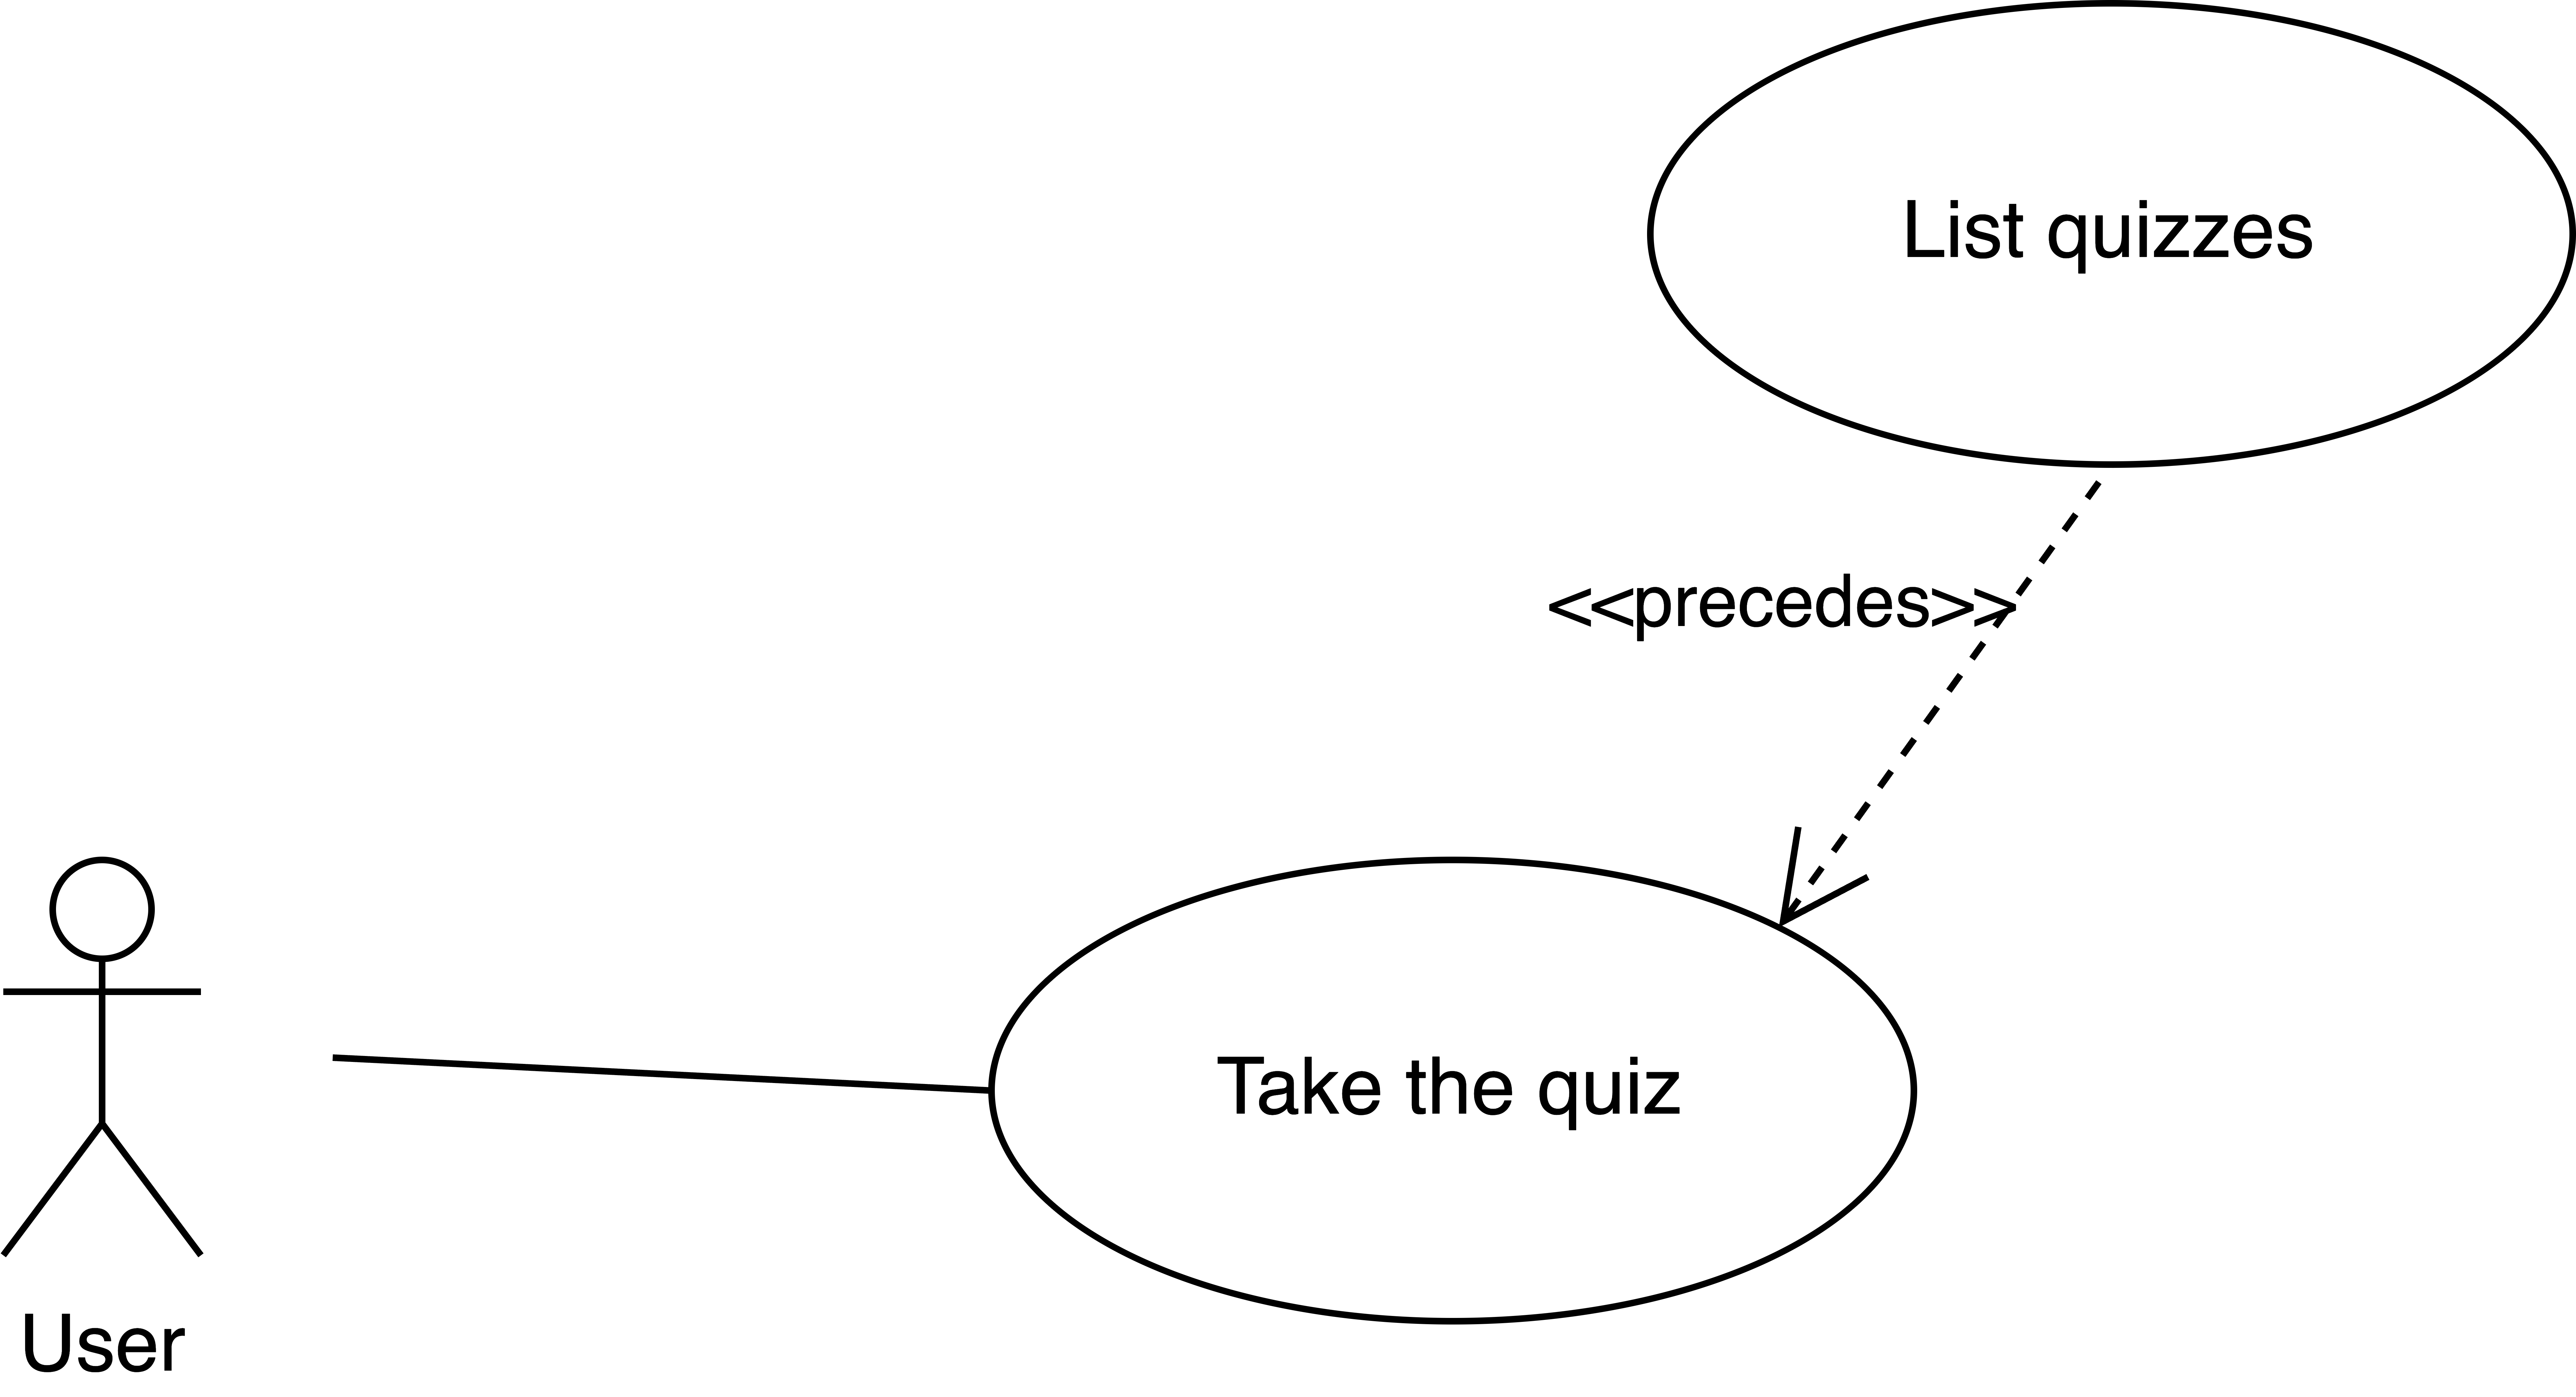
\includegraphics[width=\textwidth]{../lab3diags/take-quiz.drawio.png}
    \caption{Take quiz use case}
    \label{take-quiz}
\end{figure}

\noindent\textbf{\fontsize{13}{15}\selectfont Main scenario:}

\textit{The user} is on the particular Quiz Page. \textit{The user} clicks the p
Play Button; the system creates a \textit{quiz session} with \textit{the user}, shuffles \textit{the questions}, and displays the Question Page. \textit{The user} clicks on \textit{an option}; the system records \textit{an answer} and shows the next \textit{question}. Once \textit{the user} answers all the \textit{questions}, the system calculates the percentage of correctly answered \textit{questions} and shows the Quiz Completed Page. \textit{The user} clicks the Close Button; the system shows the Quiz Page.

\noindent\textbf{\fontsize{13}{15}\selectfont Alternatives:}

\textbf{\textit{User answer} was correct:} System displays Correct Answer Notification for 5 seconds.

\textbf{\textit{User answer} was wrong:} The system displays the Wrong Answer Page. \textit{The user} clicks on the Continue Button; and the system proceeds with the next \textit{question}.

\textbf{\textit{The user} clicks on the Restart Button on the Quiz Completed Page:} The system reshuffles \textit{the questions}, starts a new \textit{quiz session}, and shows the Question Page.

\textbf{\textit{The user} tries to leave the Question Page:} The system displays the Confirmation Popup; if \textit{the user} confirms, the system closes the page and deletes \textit{the quiz session}.

\textbf{\textit{The quiz} was edited or deleted during \textit{the session}:} The system does not show a Restart Button on the Quiz Completed Page.

\begin{figure}[ht]
    \centering
    \includegraphics[width=\textwidth]{../lab3diags/topic-owner-actions.drawio.png}
    \caption{Topic owner use cases}
    \label{topic-owner}
\end{figure}

\subsection{Delete the quiz}

\noindent\textbf{\fontsize{13}{15}\selectfont Main scenario:}

\textit{The topic owner} is on the particular Quiz Page. \textit{The topic owner} clicks on the Delete Quiz Button; the system shows a Deletion Confirmation Popup. \textit{The topic owner} clicks on the Confirm Deletion Button; the system deletes \textit{the quiz}, shows the Quiz List Page for \textit{the topic} that the deleted \textit{quiz} belonged to, and displays a Quiz Deleted Notification.

\noindent\textbf{\fontsize{13}{15}\selectfont Alternatives:}

\textbf{\textit{Topic owner} closes Confirmation Popup:} System aborts deletion.

\subsection{Create the quiz}

\noindent\textbf{\fontsize{13}{15}\selectfont Main scenario:}

\textit{The topic owner} is on the particular Quiz Page. \textit{The topic owner} clicks the Create Quiz Button; the system creates \textit{the empty quiz} in memory and shows the Quiz Editor Page associated with \textit{the quiz}. \textit{The topic owner} fills in \textit{the quiz} information and clicks the Save Quiz Button; the system saves \textit{the quiz} and shows the Quiz Page for that \textit{quiz}.

\noindent\textbf{\fontsize{13}{15}\selectfont Alternatives:}

\textbf{\textit{The topic owner} tries to leave the Quiz Editor Page:} The system displays the Confirmation Popup; if \textit{the topic owner} confirms, the system shows the Quiz List Page and removes \textit{the quiz} from memory.

\subsection{Edit the quiz}

\noindent\textbf{\fontsize{13}{15}\selectfont Main scenario:}

\textit{The topic owner} is on the particular Quiz Page. \textit{The topic owner} clicks on the Edit Button; the system shows the Quiz Editor Page associated with \textit{the quiz}. \textit{The topic owner} fills in the \textit{quiz} information and clicks the Save Quiz Button; the system saves \textit{the quiz} and shows the Quiz Page for that \textit{quiz}.

\noindent\textbf{\fontsize{13}{15}\selectfont Alternatives:}

\textbf{\textit{The topic owner} tries to leave the Quiz Editor Page:} The system displays the Confirmation Popup; if \textit{the topic owner} confirms, the system shows the Quiz List Page and aborts the changes.

\subsection{Quiz editor use cases}

Use cases here assume that \textit{the topic owner} is on the Quiz Editor Page associated with certain \textit{quiz}.

\subsubsection{Edit the quiz}

\noindent\textbf{\fontsize{13}{15}\selectfont Main scenario:}

The system shows the Quiz Editor Page. \textit{The topic owner} enters \textit{quiz} name in Quiz Name Field; system checks quiz name validity. \textit{The topic owner} clicks on the Add Question Button to add \textit{question}, the system adds a \textit{question} with no name, no image, and 2 empty \textit{options} to \textit{the quiz} and adds a Question Editor Component to the Question List on the Quiz Editor. \textit{The topic owner} clicks on the Remove Question Button to remove \textit{the question}, the system removes \textit{the question} and removes the Question Editor Component Associated with that \textit{question}. \textit{The topic owner} edits \textit{the questions} and clicks the Save Quiz Button; the system performs the action defined in the invoking use case.

\noindent\textbf{\fontsize{13}{15}\selectfont Alternatives:}

\textbf{Bad input: \textit{Quiz} has no \textit{questions}:} System shows No Questions Message near Add Question Button.

\textbf{Bad input: Text in text fields (both \textit{quiz} name and Question Components) is shorter than 5 characters or longer than 50:} The system shows a name error message near the affected text field.

\textbf{There are bad inputs:} The system disables the Save Quiz Button.

\subsubsection{Edit the question}

The correct \textit{option} is \textit{the option} on top of the Option List.

\noindent\textbf{\fontsize{13}{15}\selectfont Main scenario:}

\textit{The topic owner} enters the \textit{question} name in the Question Name Field and \textit{option} names in the Option Name Fields; the system checks the validity of the entered information. \textit{The topic owner} clicks on the Upload Image Button; the system opens the file picker. \textit{The topic owner} chooses an image file; the system downloads the image, saves it, displays the thumbnail and replaces the Add Image Button with Remove Image Button.

\noindent\textbf{\fontsize{13}{15}\selectfont Alternatives:}

\textbf{\textit{The topic owner} wants to add \textit{an option}:} \textit{The topic owner} clicks on the Add Option Button; the system adds a new empty \textit{option} at the end of the Option List.

\textbf{\textit{The topic owner} wants to remove \textit{the option}:} \textit{The topic owner} clicks on the Remove Option Button; the system removes \textit{the option}. If \textit{the option} was marked as the correct one (was on top of the list), the second \textit{option} becomes correct.

\textbf{There are 4 \textit{options}:} The system does not show the Add Option Button.

\textbf{There are 2 \textit{options}:} The system does not show the Remove Option Button

\textbf{\textit{The topic owner} wants to change the correct \textit{option}:} \textit{The topic owner} drags \textit{the option} to the top of the Option List; the system marks the dragged \textit{option} as the correct \textit{option}.

\textbf{\textit{The topic owner} wants to remove the image:} \textit{The topic owner} clicks on the Remove Image Button; the system deletes the image, removes it from the Question Component and replaces the Remove Image Button with the Add Image Button.

\section{Requirements}

\begin{description}
    \item[FR1] System shall support creation of quizzes.
    \item[FR2] System shall ensure that only owner of the topic can create, edit and delete the quiz in that topic.
    \item[FR3] System shall support editing of quizzes.
    \item[FR4] System shall support deletion of quizzes.
    \item[FR5] System shall support JPEG, PNG, SVG, WEBP, GIF image question formats.
    \item[FR6] System shall prompt for confirmation when deleting quizzes.
    \item[FR7] System shall support uploading images for questions
    \item[FR8] System shall remove uploaded images for questions of quiz being deleted.
    \item[FR9] System shall support setting quiz name.
    \item[FR10] System shall support adding, editing and deleting quiz questions and options.
    \item[FR11] System shall support listing quizzes.
    \item[FR12] System shall support users taking the quiz.
    \item[FR13] System shall check if user quiz answer was correct and notify the user.
\end{description}

\section{Traceability}

TODO: domain entities to use cases table

TODO: use cases to requirements table

\listoffigures
\printbibliography[heading=bibintoc]

\end{document}
